\chapter{Vektorrechnung}
\label{chap:vector_algebra}

Viele technische Größen besitzen neben einem Zahlenwert auch eine Richtung.
Vektoren machen beide Informationen gleichzeitig mathematisch zugänglich.

\begin{center}
  \CachedTikzFigure{content/resources/chapters/vector_algebra/tikz/scalar_vector_comparison.tex}
\end{center}

In diesem Kapitel betrachten wir Vektoren als Verschiebungspfeile im zwei- und
dreidimensionalen Raum. Dabei klären wir drei Leitfragen:
\begin{itemize}
  \item Wie werden Vektoren geometrisch und durch Koordinaten dargestellt?
  \item Wie lassen sich Vektoren addieren, subtrahieren und skalieren?
  \item Wie werden Länge und Richtung eines Vektors getrennt beschrieben?
\end{itemize}

\clearpage
\section{Grundvorstellungen und Koordinaten}
\label{sec:vector_algebra_fundamentals}

Zunächst verbinden wir die geometrische Pfeilvorstellung mit der
Koordinatendarstellung. Diese beiden Sichtweisen werden bei allen späteren
Rechenoperationen parallel verwendet.

\subsection{Vektoren als Verschiebungspfeile}
\label{subsec:vector_algebra_vectors_as_displacements}

\begin{DefinitionBox}{Vektor}{vector_algebra_vector}
  Ein \emph{Vektor} \EnglishTerm{vector} ist durch seine Länge und seine
  Richtung bestimmt. Geometrisch stellen wir ihn als
  \emph{Verschiebungspfeil} \EnglishTerm{displacement arrow} dar und schreiben
  beispielsweise $\vec a$.
  \[
    \vec a
    \quad\widehat{=}\quad
    \text{Länge und Richtung}
  \]
  Ein Vektor besitzt keine feste Position im Raum: Paralleles Verschieben
  ändert den Vektor nicht.
\end{DefinitionBox}

\begin{center}
  \CachedTikzFigure{content/resources/chapters/vector_algebra/tikz/vector_translation.tex}
\end{center}

\begin{KeyPointBox}{Beziehungen zwischen Vektoren}{vector_algebra_vector_relations}
  \noindent
  \begin{minipage}[c]{0.50\linewidth}
    \begin{align*}
      \vec a=\vec b
      &\quad\Longleftrightarrow\quad
      \text{gleiche Länge und Richtung},\\[0.6em]
      \vec a\parallel\vec b
      &\quad\Longleftrightarrow\quad
      \text{parallel oder antiparallel},\\[0.6em]
      \vec b=-\vec a
      &\quad\Longleftrightarrow\quad
      \text{Gegenvektoren}.
    \end{align*}
  \end{minipage}\hfill
  \begin{minipage}[c]{0.46\linewidth}
    \centering
    \CachedTikzFigure{content/resources/chapters/vector_algebra/tikz/vector_relations.tex}
  \end{minipage}
\end{KeyPointBox}

Der \emph{Gegenvektor} \EnglishTerm{opposite vector} zu $\vec a$ ist $-\vec a$.

\clearpage
\subsection{Koordinatendarstellung von Vektoren}
\label{subsec:vector_algebra_coordinate_representation}

In einem Koordinatensystem wird eine Verschiebung durch ihre Anteile entlang
der Koordinatenachsen beschrieben.

\begin{DefinitionBox}{Koordinaten eines Vektors}{vector_algebra_vector_coordinates}
  Ein Vektor im $n$-dimensionalen reellen Raum besitzt die
  \emph{Koordinatendarstellung} \EnglishTerm{coordinate representation}
  \[
    \vec a=
    \begin{pmatrix}
      a_1\\a_2\\\vdots\\a_n
    \end{pmatrix}
    \in\R^n.
  \]
  Die Zahl $a_i$ gibt den gerichteten Anteil von $\vec a$ entlang der
  $i$-ten Koordinatenachse an.
\end{DefinitionBox}

\noindent
\begin{minipage}[c]{0.48\linewidth}
  \[
    \vec a=\begin{pmatrix}1\\2\end{pmatrix},
    \qquad
    \vec b=\begin{pmatrix}-2\\1\end{pmatrix}
    \quad\in\R^2.
  \]
  Die Pfeile dürfen parallel verschoben werden; ihre Koordinaten bleiben
  unverändert.
\end{minipage}\hfill
\begin{minipage}[c]{0.48\linewidth}
  \centering
  \CachedTikzFigure{content/resources/chapters/vector_algebra/tikz/coordinate_vectors_2d.tex}
\end{minipage}

\begin{ExampleBox}{Vektorkoordinaten ablesen}{vector_algebra_read_coordinates}
  Die gestrichelten Hilfslinien zerlegen die Verschiebung entlang der Achsen:
  \[
    \vec a=
    \begin{pmatrix}
      \Cloze{1.2cm}{3}\\[0.35em]
      \Cloze{1.2cm}{2}
    \end{pmatrix}
    \in\R^2.
  \]
  \begin{center}
    \CachedTikzFigure{content/resources/chapters/vector_algebra/tikz/read_vector_coordinates.tex}
  \end{center}
\end{ExampleBox}

\noindent
\begin{minipage}[c]{0.43\linewidth}
  Im dreidimensionalen Raum kommt die Verschiebung entlang der $x_3$-Achse
  hinzu. Beispielsweise gilt
  \[
    \vec c=\begin{pmatrix}2\\1\\3\end{pmatrix}\in\R^3.
  \]
\end{minipage}\hfill
\begin{minipage}[c]{0.53\linewidth}
  \centering
  \CachedTikzFigure{content/resources/chapters/vector_algebra/tikz/coordinate_vector_3d.tex}
\end{minipage}

\begin{DefinitionBox}{Nullvektor}{vector_algebra_zero_vector}
  Der \emph{Nullvektor} \EnglishTerm{zero vector} besitzt ausschließlich
  Nulleinträge:
  \[
    \vec 0=
    \begin{pmatrix}0\\\vdots\\0\end{pmatrix}\in\R^n,
    \qquad
    \vec 0=\begin{pmatrix}0\\0\end{pmatrix}\in\R^2,
    \qquad
    \vec 0=\begin{pmatrix}0\\0\\0\end{pmatrix}\in\R^3.
  \]
  Er beschreibt eine Verschiebung der Länge null und besitzt keine Richtung.
\end{DefinitionBox}


\clearpage
\section{Rechnen mit Vektoren}
\label{sec:vector_algebra_operations}

Vektoren gleicher Dimension werden komponentenweise addiert und subtrahiert.
Die Multiplikation mit einer Zahl verändert ihre Länge und gegebenenfalls ihre
Richtung.

\subsection{Addition und Subtraktion}
\label{subsec:vector_algebra_addition_subtraction}

\begin{DefinitionBox}{Vektoraddition und Vektorsubtraktion}{vector_algebra_addition_subtraction}
  Für $\vec a,\vec b\in\R^n$ werden Addition und Subtraktion
  komponentenweise ausgeführt:
  \[
    \vec a+\vec b
    =\begin{pmatrix}a_1\\\vdots\\a_n\end{pmatrix}
     +\begin{pmatrix}b_1\\\vdots\\b_n\end{pmatrix}
    =\begin{pmatrix}a_1+b_1\\\vdots\\a_n+b_n\end{pmatrix},
  \]
  \[
    \vec a-\vec b
    =\vec a+(-\vec b)
    =\begin{pmatrix}a_1-b_1\\\vdots\\a_n-b_n\end{pmatrix}.
  \]
\end{DefinitionBox}

\begin{center}
  \CachedTikzFigure{content/resources/chapters/vector_algebra/tikz/vector_addition_subtraction.tex}
\end{center}

\begin{TheoremBox}{Rechenregeln der Vektoraddition}{vector_algebra_addition_laws}
  Für $\vec a,\vec b,\vec c\in\R^n$ gilt
  \[
    \begin{aligned}
      \vec a+\vec b&=\vec b+\vec a
        &&\text{(Kommutativgesetz)},\\[0.5em]
      \vec a+(\vec b+\vec c)&=(\vec a+\vec b)+\vec c
        &&\text{(Assoziativgesetz)},\\[0.5em]
      \vec a+\vec 0&=\vec a,
      &\qquad \vec a+(-\vec a)&=\vec 0.
    \end{aligned}
  \]
\end{TheoremBox}

\begin{ExampleBox}{Vektoren komponentenweise verrechnen}{vector_algebra_componentwise_operations}
  Gegeben seien
  \[
    \vec a=\begin{pmatrix}2\\0\\4\end{pmatrix},
    \qquad
    \vec b=\begin{pmatrix}-1\\2\\-10\end{pmatrix}.
  \]
  Dann gilt
  \[
    \vec a+\vec b
    =\begin{pmatrix}2+(-1)\\0+2\\4+(-10)\end{pmatrix}
    =\Cloze{3cm}{\begin{pmatrix}1\\2\\-6\end{pmatrix}},
    \qquad
    \vec a-\vec b
    =\begin{pmatrix}2-(-1)\\0-2\\4-(-10)\end{pmatrix}
    =\Cloze{3cm}{\begin{pmatrix}3\\-2\\14\end{pmatrix}}.
  \]
\end{ExampleBox}

\subsection{Multiplikation mit einem Skalar}
\label{subsec:vector_algebra_scalar_multiplication}

Eine einzelne Zahl heißt in der Vektorrechnung \emph{Skalar}
\EnglishTerm{scalar}. Sie wirkt gleichzeitig auf alle Komponenten eines
Vektors.

\begin{DefinitionBox}{Skalarmultiplikation}{vector_algebra_scalar_multiplication}
  Für $\lambda\in\R$ und $\vec a\in\R^n$ gilt
  \[
    \lambda\vec a
    =\lambda\begin{pmatrix}a_1\\a_2\\\vdots\\a_n\end{pmatrix}
    =\begin{pmatrix}\lambda a_1\\\lambda a_2\\\vdots\\\lambda a_n\end{pmatrix}.
  \]
\end{DefinitionBox}

\begin{center}
  \CachedTikzFigure{content/resources/chapters/vector_algebra/tikz/scalar_multiplication_cases.tex}
\end{center}

\begin{KeyPointBox}{Geometrische Wirkung eines Skalars}{vector_algebra_scalar_effect}
  \[
    \begin{array}{ccl}
      |\lambda|>1
      &\Longleftrightarrow&\text{Streckung},\\[0.45em]
      0<|\lambda|<1
      &\Longleftrightarrow&\text{Stauchung},\\[0.45em]
      \lambda<0
      &\Longleftrightarrow&\text{zusätzliche Richtungsumkehr},\\[0.45em]
      \lambda=0
      &\Longleftrightarrow&\lambda\vec a=\vec 0.
    \end{array}
  \]
\end{KeyPointBox}

\begin{TheoremBox}{Rechenregeln der Skalarmultiplikation}{vector_algebra_scalar_laws}
  Für $\alpha,\beta\in\R$ und $\vec a,\vec b\in\R^n$ gilt
  \[
    \begin{aligned}
      \alpha(\beta\vec a)&=(\alpha\beta)\vec a,\\[0.4em]
      (\alpha+\beta)\vec a&=\alpha\vec a+\beta\vec a,\\[0.4em]
      \alpha(\vec a+\vec b)&=\alpha\vec a+\alpha\vec b.
    \end{aligned}
  \]
\end{TheoremBox}

\begin{ExampleBox}{Einen Vektor skalieren}{vector_algebra_scale_example}
  Für $\vec a=(2,-1,3)^{\mathsf T}$ gilt
  \[
    -2\vec a
    =-2\begin{pmatrix}2\\-1\\3\end{pmatrix}
    =\Cloze{3cm}{\begin{pmatrix}-4\\2\\-6\end{pmatrix}}.
  \]
  Der Faktor $-2$ verdoppelt die Länge und kehrt die Richtung um.
\end{ExampleBox}


\clearpage
\section{Betrag, Einheitsvektoren und Standardbasis}
\label{sec:vector_algebra_magnitude_basis}

Der Betrag misst die Länge eines Vektors. Einheitsvektoren trennen anschließend
die reine Richtungsinformation von dieser Länge.

\subsection{Betrag und Einheitsvektor}
\label{subsec:vector_algebra_magnitude_unit_vectors}

\begin{DefinitionBox}{Betrag eines Vektors}{vector_algebra_vector_magnitude}
  Der \emph{Betrag} \EnglishTerm{magnitude} eines Vektors
  $\vec a=(a_1,\dots,a_n)^{\mathsf T}\in\R^n$ ist seine Länge
  \[
    |\vec a|
    =\sqrt{a_1^2+a_2^2+\dots+a_n^2}.
  \]
\end{DefinitionBox}

\noindent
\begin{minipage}[c]{0.52\linewidth}
  Für $\vec a=(3,4)^{\mathsf T}$ liefert der Satz des Pythagoras
  \[
    |\vec a|
    =\Cloze{5cm}{\sqrt{3^2+4^2}=5}.
  \]
  Für $\vec b=(1,1,1)^{\mathsf T}\in\R^3$ gilt
  \[
    |\vec b|
    =\Cloze{5cm}{\sqrt{1^2+1^2+1^2}=\sqrt3}.
  \]
\end{minipage}\hfill
\begin{minipage}[c]{0.44\linewidth}
  \centering
  \CachedTikzFigure{content/resources/chapters/vector_algebra/tikz/vector_magnitude.tex}
\end{minipage}

\begin{TheoremBox}{Rechenregeln für den Betrag}{vector_algebra_magnitude_laws}
  Für $\lambda\in\R$ und $\vec a,\vec b\in\R^n$ gilt
  \[
    |\vec a|\ge0,
    \qquad
    |\lambda\vec a|=|\lambda|\,|\vec a|,
    \qquad
    |\vec a+\vec b|\le|\vec a|+|\vec b|.
  \]
  Die letzte Beziehung heißt \emph{Dreiecksungleichung}
  \EnglishTerm{triangle inequality}.
\end{TheoremBox}

\begin{center}
  \CachedTikzFigure{content/resources/chapters/vector_algebra/tikz/triangle_inequality.tex}
\end{center}

\clearpage
\begin{DefinitionBox}{Einheitsvektor}{vector_algebra_unit_vector}
  Ein \emph{Einheitsvektor} \EnglishTerm{unit vector} $\vec e$ besitzt die
  Länge
  \[
    |\vec e|=1.
  \]
  Zu jedem $\vec a\ne\vec 0$ gehört der gleichgerichtete Einheitsvektor
  \[
    \boxed{\vec e_a=\frac{\vec a}{|\vec a|}}.
  \]
\end{DefinitionBox}

\begin{ExampleBox}{Einen Vektor normieren}{vector_algebra_normalize_vector}
  Für $\vec a=(1,1)^{\mathsf T}$ gilt
  \[
    |\vec a|=\sqrt2,
    \qquad
    \vec e_a
    =\frac{\vec a}{|\vec a|}
    =\Cloze{5cm}{\frac1{\sqrt2}\begin{pmatrix}1\\1\end{pmatrix}}.
  \]
  Damit zerfällt der Vektor in Länge und Richtung:
  \[
    \boxed{\vec a=|\vec a|\,\vec e_a}.
  \]
\end{ExampleBox}

\subsection{Koordinateneinheitsvektoren und Standardbasis}
\label{subsec:vector_algebra_standard_basis}

Entlang jeder Koordinatenachse wird ein Einheitsvektor gewählt. Diese Vektoren
bilden das Grundgerüst der Koordinatendarstellung.

\begin{DefinitionBox}{Koordinateneinheitsvektoren}{vector_algebra_coordinate_unit_vectors}
  Die \emph{Koordinateneinheitsvektoren}
  \EnglishTerm{coordinate unit vectors} lauten
  \[
    \R^2:\quad
    \vec e_1=\begin{pmatrix}1\\0\end{pmatrix},
    \quad
    \vec e_2=\begin{pmatrix}0\\1\end{pmatrix},
  \]
  \[
    \R^3:\quad
    \vec e_1=\begin{pmatrix}1\\0\\0\end{pmatrix},
    \quad
    \vec e_2=\begin{pmatrix}0\\1\\0\end{pmatrix},
    \quad
    \vec e_3=\begin{pmatrix}0\\0\\1\end{pmatrix}.
  \]
  Sie stehen paarweise senkrecht aufeinander und bilden die
  \emph{Standardbasis} \EnglishTerm{standard basis}.
\end{DefinitionBox}

\begin{center}
  \CachedTikzFigure{content/resources/chapters/vector_algebra/tikz/standard_basis.tex}
\end{center}

\begin{RemarkBox}[title=Rechtssystem]
  \label{rem:vector_algebra_right_handed_system}
  Im $\R^3$ werden die Achsen üblicherweise als \emph{Rechtssystem}
  \EnglishTerm{right-handed coordinate system} orientiert. Die gekrümmte
  Orientierung von $\vec e_1$ nach $\vec e_2$ weist dabei in Richtung
  $\vec e_3$.
  \par\smallskip
  \noindent
  \begin{minipage}[c]{0.44\linewidth}
    \centering
    \CachedTikzFigure{content/resources/chapters/vector_algebra/tikz/right_handed_basis.tex}
  \end{minipage}\hfill
  \begin{minipage}[c]{0.50\linewidth}
    \centering
    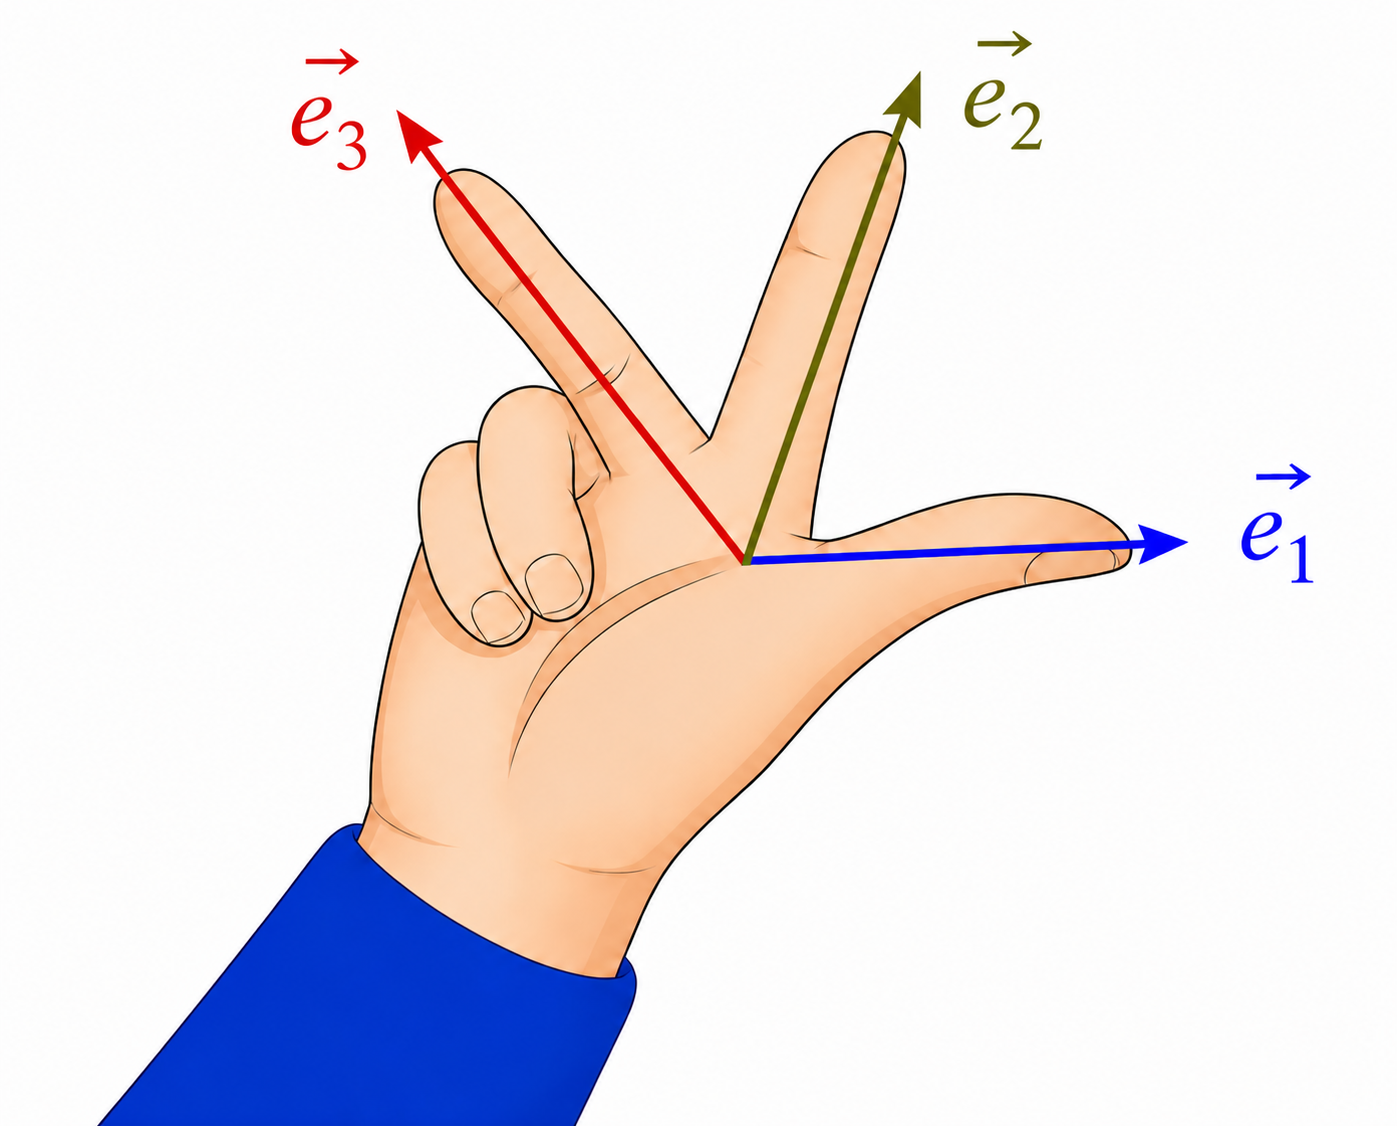
\includegraphics[width=0.68\linewidth]{content/resources/chapters/vector_algebra/images/right_handed_basis_hand.png}
  \end{minipage}
\end{RemarkBox}

\begin{KeyPointBox}{Darstellung in der Standardbasis}{vector_algebra_standard_basis_representation}
  Jeder Vektor ist die gewichtete Summe der Koordinateneinheitsvektoren:
  \[
    \R^2:\quad
    \begin{pmatrix}a_1\\a_2\end{pmatrix}
    =a_1\vec e_1+a_2\vec e_2,
    \qquad
    \R^3:\quad
    \begin{pmatrix}a_1\\a_2\\a_3\end{pmatrix}
    =a_1\vec e_1+a_2\vec e_2+a_3\vec e_3.
  \]
\end{KeyPointBox}

\begin{ExampleBox}{Koordinaten als Gewichte der Basisvektoren}{vector_algebra_basis_decomposition}
  \[
    \begin{pmatrix}2\\3\end{pmatrix}
    =\Cloze{6cm}{2\vec e_1+3\vec e_2},
    \qquad
    \begin{pmatrix}1\\2\\3\end{pmatrix}
    =\Cloze{8cm}{\vec e_1+2\vec e_2+3\vec e_3}.
  \]
\end{ExampleBox}


\clearpage
\section{Skalarprodukt}
\label{sec:vector_algebra_scalar_product}

Das Skalarprodukt verknüpft zwei Vektoren mit einer Zahl. Dadurch werden
Winkel, Orthogonalität, Projektionen und Längen von Vektorkombinationen
rechnerisch zugänglich.

\subsection{Geometrische Definition}
\label{subsec:vector_algebra_scalar_product_definition}

\begin{DefinitionBox}{Skalarprodukt}{vector_algebra_scalar_product}
  Für zwei von null verschiedene Vektoren $\vec a,\vec b\in\R^n$ und den
  eingeschlossenen Winkel $0\le\varphi\le\pi$ ist das
  \emph{Skalarprodukt} \EnglishTerm{dot product} definiert durch
  \[
    \boxed{\vec a\cdot\vec b=|\vec a|\,|\vec b|\cos(\varphi)}.
  \]
  Für den Nullvektor wird $\vec a\cdot\vec 0=\vec 0\cdot\vec a=0$ gesetzt.
\end{DefinitionBox}

\noindent
\begin{minipage}[c]{0.49\linewidth}
  \centering
  \CachedTikzFigure{content/resources/chapters/vector_algebra/tikz/dot_product_geometry.tex}
\end{minipage}\hfill
\begin{minipage}[c]{0.47\linewidth}
  \begin{KeyPointBox}{Das Ergebnis ist ein Skalar}{vector_algebra_dot_product_scalar}
    \[
      \underbrace{\vec a}_{\text{Vektor}}
      \cdot
      \underbrace{\vec b}_{\text{Vektor}}
      =
      \underbrace{s}_{\text{Skalar}}\in\R.
    \]
    Das Skalarprodukt ist kein Vektor und wird nicht komponentenweise als
    Vektor ausgegeben.
  \end{KeyPointBox}
\end{minipage}

\begin{ExampleBox}{Skalarprodukt aus Längen und Winkel}{vector_algebra_geometric_dot_product_example}
  Für $|\vec a|=2$, $|\vec b|=3$ und $\varphi=30^\circ$ gilt
  \[
    \vec a\cdot\vec b
    =2\cdot3\cdot\cos(30^\circ)
    =\Cloze{4cm}{3\sqrt3}.
  \]
\end{ExampleBox}

\begin{KeyPointBox}{Vorzeichen und eingeschlossener Winkel}{vector_algebra_dot_product_sign}
  \begin{center}
    \CachedTikzFigure{content/resources/chapters/vector_algebra/tikz/dot_product_signs.tex}
  \end{center}
\end{KeyPointBox}

\subsection{Rechenregeln}
\label{subsec:vector_algebra_scalar_product_rules}

\begin{TheoremBox}{Rechenregeln des Skalarprodukts}{vector_algebra_dot_product_laws}
  Für $\vec a,\vec b,\vec c\in\R^n$ und $\lambda\in\R$ gilt
  \[
    \begin{aligned}
      \vec a\cdot\vec b
        &=\vec b\cdot\vec a
        &&\text{(Kommutativgesetz)},\\[0.5em]
      \vec a\cdot(\vec b+\vec c)
        &=\vec a\cdot\vec b+\vec a\cdot\vec c
        &&\text{(Distributivgesetz)},\\[0.5em]
      (\lambda\vec a)\cdot\vec b
        &=\lambda(\vec a\cdot\vec b)
        =\vec a\cdot(\lambda\vec b).
    \end{aligned}
  \]
\end{TheoremBox}

\begin{RemarkBox}[title=Keine Assoziativität]
  \label{rem:vector_algebra_dot_product_not_associative}
  Ein Assoziativgesetz ist nicht möglich: $\vec a\cdot\vec b$ ist bereits
  ein Skalar. Daher sind $(\vec a\cdot\vec b)\cdot\vec c$ und
  $\vec a\cdot(\vec b\cdot\vec c)$ keine Skalarprodukte zweier Vektoren.
\end{RemarkBox}

\begin{ExampleBox}{Rechenregeln anwenden}{vector_algebra_dot_product_laws_example}
  Für
  \[
    \vec a=\begin{pmatrix}1\\2\end{pmatrix},\qquad
    \vec b=\begin{pmatrix}3\\-1\end{pmatrix},\qquad
    \vec c=\begin{pmatrix}-1\\4\end{pmatrix}
  \]
  folgt
  \[
    \vec a\cdot(\vec b+\vec c)
    =\vec a\cdot\vec b+\vec a\cdot\vec c
    =\Cloze{5cm}{1+7=8}.
  \]
\end{ExampleBox}

\clearpage
\subsection{Skalarprodukt in Koordinatendarstellung}
\label{subsec:vector_algebra_dot_product_coordinates}

Nun suchen wir noch eine Formel, um das Skalarprodukt zweier Vektoren,
die in ihrer Koordinatenform vorliegen zu berechnen. Diese Formel heißt
Koordinatenformel des Skalarprodukts.
Dazu stellen wir zunächst die zwei Vektoren $\vec a,\vec b\in\R^3$ mit
den kanonischen Einheitsvektoren dar:
\[
  \begin{aligned}
    \vec a
      &=\Cloze{10cm}{a_1\vec e_1+a_2\vec e_2+a_3\vec e_3},\\[1em]
    \vec b
      &=\Cloze{10cm}{b_1\vec e_1+b_2\vec e_2+b_3\vec e_3}.
  \end{aligned}
\]

Die kanonischen Einheitsvektoren sind orthonormal, d.h. sie sind 
paarweise senkrecht und haben den Betrag $1$. Daher gilt
\[
  \vec e_i\cdot\vec e_j
  =\begin{cases}
     1,&i=j,\\
     0,&i\ne j.
   \end{cases}
\]

Durch Einsetzen in das Skalarprodukt und anschliendes Ausmultiplizieren erhalten wir
\begin{ClozeArea}[34]{10}
  \[
    \begin{aligned}
      \vec a\cdot\vec b
      &=(a_1\vec e_1+a_2\vec e_2+a_3\vec e_3)
        \cdot(b_1\vec e_1+b_2\vec e_2+b_3\vec e_3)
        \vphantom{\overbrace{(\vec e_1\cdot\vec e_1)}^{=1}}\\[0.7em]
      &=a_1b_1\overbrace{(\vec e_1\cdot\vec e_1)}^{=1}
        +a_1b_2\overbrace{(\vec e_1\cdot\vec e_2)}^{=0}
        +a_1b_3\overbrace{(\vec e_1\cdot\vec e_3)}^{=0}\\[0.7em]
      &\quad
        +a_2b_1\overbrace{(\vec e_2\cdot\vec e_1)}^{=0}
        +a_2b_2\overbrace{(\vec e_2\cdot\vec e_2)}^{=1}
        +a_2b_3\overbrace{(\vec e_2\cdot\vec e_3)}^{=0}\\[0.7em]
      &\quad
        +a_3b_1\overbrace{(\vec e_3\cdot\vec e_1)}^{=0}
        +a_3b_2\overbrace{(\vec e_3\cdot\vec e_2)}^{=0}
        +a_3b_3\overbrace{(\vec e_3\cdot\vec e_3)}^{=1}\\[0.7em]
      &=a_1b_1+a_2b_2+a_3b_3
        \vphantom{\overbrace{(\vec e_1\cdot\vec e_1)}^{=1}}.
    \end{aligned}
  \]
\end{ClozeArea}

\begin{TheoremBox}{Koordinatenformel des Skalarprodukts}{vector_algebra_dot_product_coordinate_formula}
  Für das Skalarprodukt zweier Vektoren $\vec a,\vec b\in\R^n$ gilt
  \[
    \vec a\cdot\vec b
    =\begin{pmatrix}
      a_1\\a_2\\\vdots\\a_n
    \end{pmatrix}
    \cdot
    \begin{pmatrix}
      b_1\\b_2\\\vdots\\b_n
    \end{pmatrix}
    =a_1b_1+a_2b_2+\dots+a_nb_n
    =\sum_{i=1}^{n}a_i b_i.
  \]
  Komponenten mit gleichem Index werden multipliziert und anschließend werden
  die Produkte addiert.
\end{TheoremBox}

\begin{ExampleBox}{Skalarprodukt aus Koordinaten}{vector_algebra_coordinate_dot_product_example}
  \begin{enumerate}[label=\alph*),leftmargin=1.8em,itemsep=1em]
    \item
      \(\displaystyle
        \begin{pmatrix}1\\2\end{pmatrix}
        \cdot
        \begin{pmatrix}3\\4\end{pmatrix}
        =\Cloze{5cm}{1\cdot3+2\cdot4=11}.
      \)

    \item
      \(\displaystyle
        \begin{pmatrix}1\\2\\3\end{pmatrix}
        \cdot
        \begin{pmatrix}4\\5\\6\end{pmatrix}
        =\Cloze{7cm}{1\cdot4+2\cdot5+3\cdot6=32}.
      \)
  \end{enumerate}
\end{ExampleBox}

\subsection{Orthogonalität und Winkel}
\label{subsec:vector_algebra_orthogonality_angles}

\begin{KeyPointBox}{Orthogonalitätskriterium}{vector_algebra_orthogonality_criterion}
  Zwei von null verschiedene Vektoren sind genau dann
  \emph{orthogonal} \EnglishTerm{orthogonal}, wenn ihr Skalarprodukt null ist:
  \[
    \boxed{\vec a\perp\vec b\quad\Longleftrightarrow\quad
      \vec a\cdot\vec b=0}.
  \]
\end{KeyPointBox}

\begin{ExampleBox}{Eine orthogonale Richtung bestimmen}{vector_algebra_find_orthogonal_vector}
  Für
  \[
    \vec a=\begin{pmatrix}1\\2\end{pmatrix},
    \qquad
    \vec b=\begin{pmatrix}4\\x\end{pmatrix}
  \]
  soll $\vec a\perp\vec b$ gelten. Dann
  \[
    \vec a\cdot\vec b=0
    \quad\Longleftrightarrow\quad
    4+2x=0
    \quad\Longleftrightarrow\quad
    x=\Cloze{2cm}{-2}.
  \]
  \begin{center}
    \CachedTikzFigure{content/resources/chapters/vector_algebra/tikz/orthogonal_vectors_example.tex}
  \end{center}
\end{ExampleBox}

\begin{KeyPointBox}{Winkel zwischen zwei Vektoren}{vector_algebra_angle_between_vectors}
  Für $\vec a,\vec b\ne\vec 0$ folgt aus der geometrischen Definition
  \[
    \cos(\varphi)=\frac{\vec a\cdot\vec b}{|\vec a|\,|\vec b|}
    \qquad\Longrightarrow\qquad
    \boxed{
      \varphi=\arccos\!\left(
        \frac{\vec a\cdot\vec b}{|\vec a|\,|\vec b|}
      \right)
    }.
  \]
\end{KeyPointBox}

\begin{ExampleBox}{Winkel zweier Vektoren}{vector_algebra_angle_example}
  \noindent
  \begin{minipage}[c]{0.56\linewidth}
    Für $\vec a=(1,2)^{\mathsf T}$ und
    $\vec b=(4,0)^{\mathsf T}$ gilt
    \[
      \vec a\cdot\vec b=4,
      \quad |\vec a|=\sqrt5,
      \quad |\vec b|=4,
    \]
    \[
      \varphi
      =\arccos\!\left(\frac{4}{4\sqrt5}\right)
      =\Cloze{4cm}{\arccos\!\left(\frac1{\sqrt5}\right)
        \approx63{,}4^\circ}.
    \]
  \end{minipage}\hfill
  \begin{minipage}[c]{0.40\linewidth}
    \centering
    \CachedTikzFigure{content/resources/chapters/vector_algebra/tikz/angle_between_vectors_example.tex}
  \end{minipage}
\end{ExampleBox}

\clearpage
\subsection{Orthogonale Projektion}
\label{subsec:vector_algebra_orthogonal_projection}

Ein Vektor $\vec b$ lässt sich relativ zu einer Richtung $\vec a\ne\vec 0$
in eine parallele und eine senkrechte Komponente zerlegen:
\[
  \boxed{\vec b=\vec b_{\parallel}+\vec b_{\perp}}.
\]

\begin{center}
  \CachedTikzFigure{content/resources/chapters/vector_algebra/tikz/orthogonal_projection.tex}
\end{center}

Mit dem Einheitsvektor $\vec e_a=\vec a/|\vec a|$ ergibt sich die
vorzeichenbehaftete Komponente von $\vec b$ in Richtung $\vec a$:
\begin{ClozeArea}[34]{5}
  \[
    \begin{aligned}
      \vec b\cdot\vec e_a
      &=(\vec b_{\parallel}+\vec b_{\perp})\cdot\vec e_a\\[0.5em]
      &=\vec b_{\parallel}\cdot\vec e_a
        +\underbrace{\vec b_{\perp}\cdot\vec e_a}_{=0}.
    \end{aligned}
  \]
\end{ClozeArea}

\begin{KeyPointBox}{Parallele und senkrechte Komponente}{vector_algebra_projection_components}
  \[
    \boxed{
      \vec b_{\parallel}
      =(\vec b\cdot\vec e_a)\,\vec e_a
      =\frac{\vec a\cdot\vec b}{\vec a\cdot\vec a}\,\vec a
    },
  \]
  \[
    \boxed{
      \vec b_{\perp}
      =\vec b-\vec b_{\parallel}
    }.
  \]
  Dabei gilt $|\vec b_{\parallel}|=|\vec b\cdot\vec e_a|$ und
  $\vec a\cdot\vec b_{\perp}=0$.
\end{KeyPointBox}

\begin{ExampleBox}{Einen Vektor orthogonal zerlegen}{vector_algebra_projection_example}
  Gegeben seien
  \[
    \vec a=\begin{pmatrix}2\\1\end{pmatrix},
    \qquad
    \vec b=\begin{pmatrix}1\\3\end{pmatrix}.
  \]
  Dann gilt
  \[
    \vec b_{\parallel}
    =\frac{\vec a\cdot\vec b}{\vec a\cdot\vec a}\,\vec a
    =\frac5{5}\begin{pmatrix}2\\1\end{pmatrix}
    =\Cloze{2.5cm}{\begin{pmatrix}2\\1\end{pmatrix}},
  \]
  \[
    \vec b_{\perp}
    =\vec b-\vec b_{\parallel}
    =\Cloze{2.5cm}{\begin{pmatrix}-1\\2\end{pmatrix}},
    \qquad
    \vec a\cdot\vec b_{\perp}=0.
  \]
\end{ExampleBox}

\clearpage
\subsection{Betrag von Summen und Differenzen}
\label{subsec:vector_algebra_magnitude_sums_differences}

Das Skalarprodukt macht sichtbar, wie der eingeschlossene Winkel den Betrag
von $\vec a+\vec b$ beziehungsweise $\vec a-\vec b$ beeinflusst.

\begin{center}
  \CachedTikzFigure{content/resources/chapters/vector_algebra/tikz/vector_sum_difference_magnitudes.tex}
\end{center}

Für $\vec a,\vec b\ne\vec 0$ und den eingeschlossenen Winkel $\varphi$ gilt:
\begin{ClozeArea}[34]{7}
  \[
    \begin{aligned}
      |\vec a\pm\vec b|^2
      &=(\vec a\pm\vec b)\cdot(\vec a\pm\vec b)\\[0.5em]
      &=\vec a\cdot\vec a+\vec b\cdot\vec b
        \pm2\,\vec a\cdot\vec b\\[0.5em]
      &=|\vec a|^2+|\vec b|^2
        \pm2|\vec a|\,|\vec b|\cos(\varphi).
    \end{aligned}
  \]
\end{ClozeArea}

\begin{KeyPointBox}{Beträge von Vektorkombinationen}{vector_algebra_sum_difference_magnitudes}
  \[
    \boxed{
      |\vec a\pm\vec b|
      =\sqrt{|\vec a|^2+|\vec b|^2
        \pm2|\vec a|\,|\vec b|\cos(\varphi)}
    }.
  \]
\end{KeyPointBox}

\begin{KeyPointBox}{Kosinussatz als Differenzfall}{vector_algebra_cosine_rule_derivation}
  Bilden $\vec a$ und $\vec b$ zwei Dreiecksseiten mit gemeinsamem
  Anfangspunkt und ist $\vec c=\vec a-\vec b$, so folgt unmittelbar
  \[
    \boxed{c^2=a^2+b^2-2ab\cos(\varphi)}.
  \]
  Für $\varphi=90^\circ$ bleibt der Satz des Pythagoras.
\end{KeyPointBox}

\begin{ExampleBox}{Differenz zweier gleich langer Vektoren}{vector_algebra_difference_magnitude_example}
  Für $|\vec a|=|\vec b|=\qty{3}{\centi\meter}$ und
  $\varphi=30^\circ$ gilt
  \[
    |\vec a-\vec b|^2
    =(\qty{3}{\centi\meter})^2+(\qty{3}{\centi\meter})^2
    -2(\qty{3}{\centi\meter})(\qty{3}{\centi\meter})\cos(30^\circ),
  \]
  \[
    |\vec a-\vec b|
    =\Cloze{5cm}{\sqrt{18-9\sqrt3}\,\unit{\centi\meter}
      \approx\qty{1.55}{\centi\meter}}.
  \]
\end{ExampleBox}


